\documentclass{llncs}
\usepackage[utf8]{inputenc}
\usepackage[T1]{fontenc}
\usepackage{fixltx2e}
\usepackage{graphicx}
\usepackage{grffile}
\usepackage{longtable}
\usepackage{wrapfig}
\usepackage{rotating}
\usepackage[normalem]{ulem}
\usepackage{amsmath}
\usepackage{textcomp}
\usepackage{amssymb}
\usepackage{capt-of}
\usepackage{hyperref}
\usepackage{makeidx}  % allows for indexgeneration
\title{Toward a Model of Surface Story Content in Cinematic Choice-Based Adventure Games}
\hypersetup{
 pdfauthor={John Murray},
 pdftitle={Toward a Model of Surface Story Content in Cinematic Choice-Based Adventure Games},
 pdfkeywords={},
 pdfsubject={},
 pdflang={English}}
\begin{document}

\maketitle
\begin{abstract}
\label{sec:orgheadline1}
We present a description of a preliminary schema and prototype of an approach to encoding the surface story content of a subgenre of interactive narratives, cinematic choice-based adventure games. The prototype and proposed work is to document the surface structure of a published game, The Wolf Among Us by Telltale Games. The proposed encoding capture the salient features of existing cinematic branching narratives relevant to the interpretation of story, in particular the sequence and the logic of the traversals, and makes it available for deeper modeling and analysis. One goal for the proposed interface is to understand complex relationships between selection and presentation of content and the experience players have in making choices. Future work includes encoding the complete work and using that to understand how interactive narratives can be modeled using models of narrative discourse such as David Elson's Story Intention Graphs \cite{Elson2012}.

\keywords\{Intelligent Narrative Technologies, Computational analysis
of narratives, Interactive cinema and television\}
\end{abstract}
\section*{Introduction}
\label{sec:orgheadline2}
Contemporary interactive narratives such as Telltale Games \emph{The Wolf
Among Us} use a combination of cinematic tropes and choice-based
mechanics to create unique player experiences around story. This paper
describes an approach to encoding the surface content in such a way as
to preserve the logic and the essential structures relevant to its
role in conveying the story.

Interactive digital narratives represent a possibility space of
potential stories which require non-trivial effort to "experience."
Espen Aarseth calls these works "ergodic literature" in his book,
\emph{Cybertext} \cite{Aarseth1997}, drawing attention to the properties
that differentiates this medium from other types of literature. Nick
Montfort uses the term "traversal" \footnote{In interactive fiction, this is a textual transcript as all
input and output of the work is recorded in a log.} to describe one possible or
actual story that results from engaging with a work, further
distinguishing "successful" or "complete" traversals based on
completion.  For instance, a failure of the player to overcome an
obstacle, resulting in the character's death, does not always result
in completion of the intended story content, but rather requires the
player to attempt the challenge again before proceeding
\cite{Montfort2006}. Hartmut Koenitz proposed the term "instance" to
describe a parameterized traversal, using the sense prevalent in
computer programming \cite{Hartmut2015}.  Koenitz describes the space
of instances as a "protostory." We will use the term "traversal" to
refer to a sequence of player actions and initial encounter of story
content. This definition allows us to remain focused on the story
content without getting distracted by the totality of possible
executions and user inputs that would be possible with an interactive
program, especially one which has sections that allow the player to
remain indefinitely or to revisit content infinitely.

This paper describes an approach to measuring, recording, and
exploring the surface traversals of a subgenre of interactive
narratives. It takes a very evidence-based approach to support future
theories and computational models. 

The proposed encoding and prototype addresses the following research
question:

\begin{quote}
How do you define and represent, using story control logics, the
significant story-related surface content of cinematic choice-based
adventure games?
\end{quote}

After defining the subgenre of interest and why it is suitable, we
will describe the specific proposed elements of the surface encoding,
followed by a method to evaluate them as future work.

\section*{Cinematic Choice-based Adventure Games}
\label{sec:orgheadline3}
Telltale Game’s \emph{The Wolf Among Us} was released in 2013 for multiple
platforms. The game received numerous positive critical reviews and
represents a mature example of this subgenre. Its story content is
conveyed through a combination of dialogue, performance of the
characters and cinematography. The game has even been translated into
a comic book, the original media that of the \emph{Fables} series on which
the game is based \cite{Sturges2014}. 

The label "cinematic choice-based adventure game" was chosen not
because it is the popular name used for this subgenre of adventure
games, which could be considered a hybrid of the point-and-click
adventure game and interactive movie, but rather for how it highlights
the primary mechanics (making choices) and the primary
representational mode (cinematic) as well as including the historical
genre of adventure games which is distinguished by distinct authored
player-character(s) and an emphasis on story.

The player's choices vary the way in which that performance is
carried out as well as certain key facts that make up the plot. Most
decisions and actions only have an impact on the pacing or variation
of the performance rather than ontological changes in the plot, such
as the timing for choosing menu options or choosing two options that
have the same outcome but which have apparent different descriptive
text. Some choices result in content which provides the player
satisfaction later in the game, labeled the "payoff" in this
document. Another term that will be useful is the concept of an
"influential thread", or content that plays a role in affecting a
future player decision.

Cinematic choice-based adventure games avoid themed puzzles such as
the cake puzzle in Graeme Devine's \emph{7th Guest}, coordination skill
tests such as the various object and physics puzzles in Valve's
\emph{Portal} or abstract logic puzzles such as found in Jonathan Blow's
\emph{The Witness}. Instead, the subgenre favors dramatically staged
choices that branch the story's presentation, making it an ideal
candidate for modeling the surface story content in the context of a
specific subset of operational logics that overlap with interface and
performance logics.

By conserving content and maximizing payoffs among possible
traversals, this subgenre is ideally suited to algorithmic traversal
by the intentional frames captured by SIGs, as the player’s goals and
intentions are rewarded while the story remains relatively consistent.

\section*{Story Control Logics}
\label{sec:orgheadline9}
Noah Wardrip-Fruin introduced the analytical concept of operational
logics \cite{Wardrip-fruin} to describe the synergistic relationship
of abstract process and representational goals. He did so in the
context of understanding the relationships between surface, process
and data in the work leading up to the book \emph{Expressive Processing},
and described some of the key insights there \cite{Wardrip-Fruin2009}.
The concept was later formalized and further defined in collaboration
with Michael Mateas in \cite{Mateas2009b}:

\begin{quote}
An operational logic defines an authoring (representational)
strategy, supported by abstract processes or lower-level logics, for
specifying the behaviors a system must exhibit in order to be
understood as representing a specified domain to a specified
audience. \cite{Mateas2009b}
\end{quote}

Operational logics can be used to precisely model and analyze how an
author communicates through a set of abstract processes and
representations an underlying "domain" with an audience. This
proposal's surface content model depends on the slipperiness of the
domain of human affairs that is narrative, and how at the same time
operational logics "determine the state evolution of a system," how
they specify an abstract model of the underlying system, "with how
they are understood at a human level," through the proposed encoding
\cite{Mateas2009b}. 

The proposed encoding of the surface representation depends on a model
of the underlying operations that each of the proposed story control
logics. These logics occupy the intersection between (graphical)
interface logics and performance logics, as they provide the player
with options tied to an underlying content selection architecture as
well as afford the player a set of performance options that either
determine or enact the choices.

The state evolution and representational strategy of cinematic
choice-based adventure games is represented by modeling the following
\textbf{story control logics}:

\begin{center}
\begin{tabular}{ll}
Operational Logic Name & Description\\
\hline
\textbf{1} \emph{Response Selection} & Language-based menus that reflect player-character options.\\
\textbf{2} \emph{Object-Verb Selections} & Verb-selection for object or character.\\
\textbf{3} \emph{Inventory} & Objects that either reflect ongoing or past plots\\
\textbf{4} \emph{Quick-time} & Affordances that require enactment to proceed\\
\textbf{5} /"Payoff" Signaling/ & Text that indicates (truthfully or not) underlying state\\
\end{tabular}
\end{center}

There are other operational logics at work, such as collision logics
and camera control logics, but these don't affect the story structure
as defined by the SIG. The five above operational logics cover every
relevant non-linear control mechanism and corresponding
representation. These logics must be in a surface model in order to
represent the possible variations. 

\subsection*{Response Selection}
\label{sec:orgheadline4}
\textbf{Response selection} logic is, like the others, a genre of interface
logic. It is how a player selects the next actions or intent of the
character. Like most adventure games, the player-character carries out
the action or dialogue in their characteristic way. The underlying
operation is simply one of selecting the content to be played.

\subsection*{Object-Verb Selection Logics}
\label{sec:orgheadline5}
This logic is a variant on the response selection, except that it
plays the character interacting with an object instead of interacting
with a character and often has physical actions instead of dialogue
options. An example is either knocking or kicking down a door, or
picking up an object.

\subsection*{Inventory Logics}
\label{sec:orgheadline6}
In this logic, the main function is to track whether certain content
choices are available for selection. Secondarily, it is a reminder of
important plot threads.
\subsection*{Quick-time Logics}
\label{sec:orgheadline7}
This represents the enactment of the player of a particular situation
the character is in, often through repeated button presses or through
a quick decision in a heated moment. It can be considered a subtype of
performance logics. Failing these may result in replaying from a
checkpoint, so most do not branch the story.
\subsection*{"Payoff" signaling}
\label{sec:orgheadline8}
This is one of the more complex operational logics that communicates a
possible underlying state that may not be modeled at the system level
at all. Instead, the text may shape player expectations of how their
decision affected agents or could result in future opportunities. It
is because of this expectation that it needs to be represented as a
distinct logic in the surface story content, and because it is
consistently applied in a way that would suggest an underlying model
is being affected.

The complexity of navigating the surface content defined by these
logics and the recorded gameplay motivates the creation of a "story
browser" tool to aid analyzing the distribution and patterns that the
content takes.
\section*{Proposed Encoding Elements}
\label{sec:orgheadline14}
\subsection*{Timecodes}
\label{sec:orgheadline10}
In film, a timecode is a way to uniquely identify every frame in a
piece of video. The format is similar to traditional time
representations, with hour, minute and second separated by colons. In
addition, this format includes the frame, which for the purposes of
this study will be at a framerate of 30 frames per second.

This means a format of 05:04:10 represents a frame at 5 minutes, 4
seconds and 10 frames, or frame number 9120.

Because this study considers non-linear games, the gameplay footage
cannot be simply mapped to traditional timecodes. Instead, the
gameplay is divided into segments roughly corresponding to cutscenes
and interaction opportunities. These are detailed in the following
sections.

\subsection*{Shots and Segments}
\label{sec:orgheadline11}
In film studies, a shot by shot analysis usually divides film into
continuous sequences of frames which are separated by cuts or other
transitions. In this format, shots are identified by timecode and made
available for tagging as a semantic unit.

Sequences of shots are further aggregated into segments which indicate
key boundaries that are bounded by opportunities for interaction.

The proposed methods of dealing with this type of content is to
identify each segment uniquely and describe the relationship both to
the preceding and succeeding segments as well as the logical
conditions under which that segment is both shown and made available
(as in the case of choices where a certain condition must have been
met in order for a choice to be available).

This is a breakdown of the beginning portion of a single source file
into shots, showing the timecode for the start and end and the unique
ID used elsewhere.

\begin{verbatim}
[
    {
        "shot_id": 0,
        "thumb" : null,
        "source_file" : "source_1",
        "source_begin" : "00:00:00",
        "source_end" : "00:08:18",
    },
]
\end{verbatim}

A segment is simply a set of shots that either are between, during or
result from a player action. This technique requires a different
tactic for free-roam segments (an example walkthrough for each
hotspot, for instance), but includes quick-time segments.

\begin{verbatim}
[
  {
    "segment_id": 0,
    "type": "cutscene",
    "begin": "00:00:00",
    "end": "01:52:22",
    "thumb": null,
      "shots": [0,1,2,3,4,5,6,7,8,9,
                10,11,12,13,14,15,16,
                17,18],
    "beats": []
  },
  {
    "segment_id": 1,
      "type": "choice",
      "choices_id":0,
      "begin": "01:52:23",
      "end": "02:24:29",
      "predecessors":[0],
      "thumb": null,
      "shots": [19,20,21,22,23],
      "beats": []
  }
]
\end{verbatim}
\subsection*{Choice Points}
\label{sec:orgheadline12}
"Choice Points" are the segments where a (usually textual) menu of
responses are presented for the player to make a decision. They
usually consist of either a paraphrase of the response but can include
either silence or an action in brackets. Selecting an option triggers
a segment which dramatically presents how that choice plays out,
usually first by an action or a dialogue act by the player-character
(Bigby Wolf in \emph{The Wolf Among Us}), followed by the response by
another character or character(s) and/or the environment.

Choice points represent a particularly important feature of the
encoded surface content. The data structure reflects both the role as
variable (each choice determines which future choices are available)
as well as preconditions (some choices requires that certain
conditions be met in order to be present in a set of choices).

This is a possible data structure that captures the graph nature as
well as the text necessary for rendering interfaces. It has an ID of
the associated segment that plays during the choice itself as well as
access to the text of the choice. Further additions would be
pre-conditions such as presence or absence of an inventory item or a
previous choice the player made.

\begin{verbatim}
[{
		"segment_id": 5,
		"choices": [{
			"alt_id": 0,
			"choice_text": "So what have I walked into?",
			"next_segment": 7
		}, {
			"alt_id": 1,
			"choice_text": "What do you want me to do?",
			"next_segment": 7
		}, {
			"alt_id": 2,
			"choice_text": "[Head Upstairs]",
			"next_segment": 8
		}, {
			"alt_id": 3,
			"choice_text": "...",
			"next_segment": 7
		}]
	}]
\end{verbatim}

Likewise, for quicktime events they would indicate the type, duration
and the action sequence in the same way that choices did.

\begin{verbatim}
[{
		"quicktime_event": {
			"key": "up"
		}
	}, {
		"quicktime_choice": {
			"choices": [{
				"alt_id": 0,
				"description": "couch",
				"mouse": "left"
			}, {
				"alt_id": 1,
				"description": "sink",
				"mouse": "left"
			}]
		}
	}]
\end{verbatim}
\subsection*{Dialogue}
\label{sec:orgheadline13}
Another key content represented in this format is the dialogue. This
represents textual content, but it is usually for a full listing of
different structures supported and the types of information each
encodes. Below is a sample of some dialogue encoded for the first
scene:

For dialogue and other text, we plan to use the industry standard VTT
encoding which is used for subtitles and captions for video
content. Below is a sample of the encoding at work.

\begin{verbatim}
[
    {
        "lineid": 9,
        "type": "dialogue",
        "begin": "1:56:01",
        "end": "1:56:29",
        "speaker": "bigby",
        "text": "Mr. Toad?"
    },
]
\end{verbatim}

\section{Story Browser Prototype}
\label{sec:orgheadline15}
The browser demonstrates the basic approach taken in the system
provide a set of parallel encodings of content locations that can be
used as various layers of surface discourse. Allow this content to be
rearranged according to the structural characteristics of the
underlying operational logic in the game, in particular choice points,
inventory items, decisions.

\begin{figure}[htb]
\centering
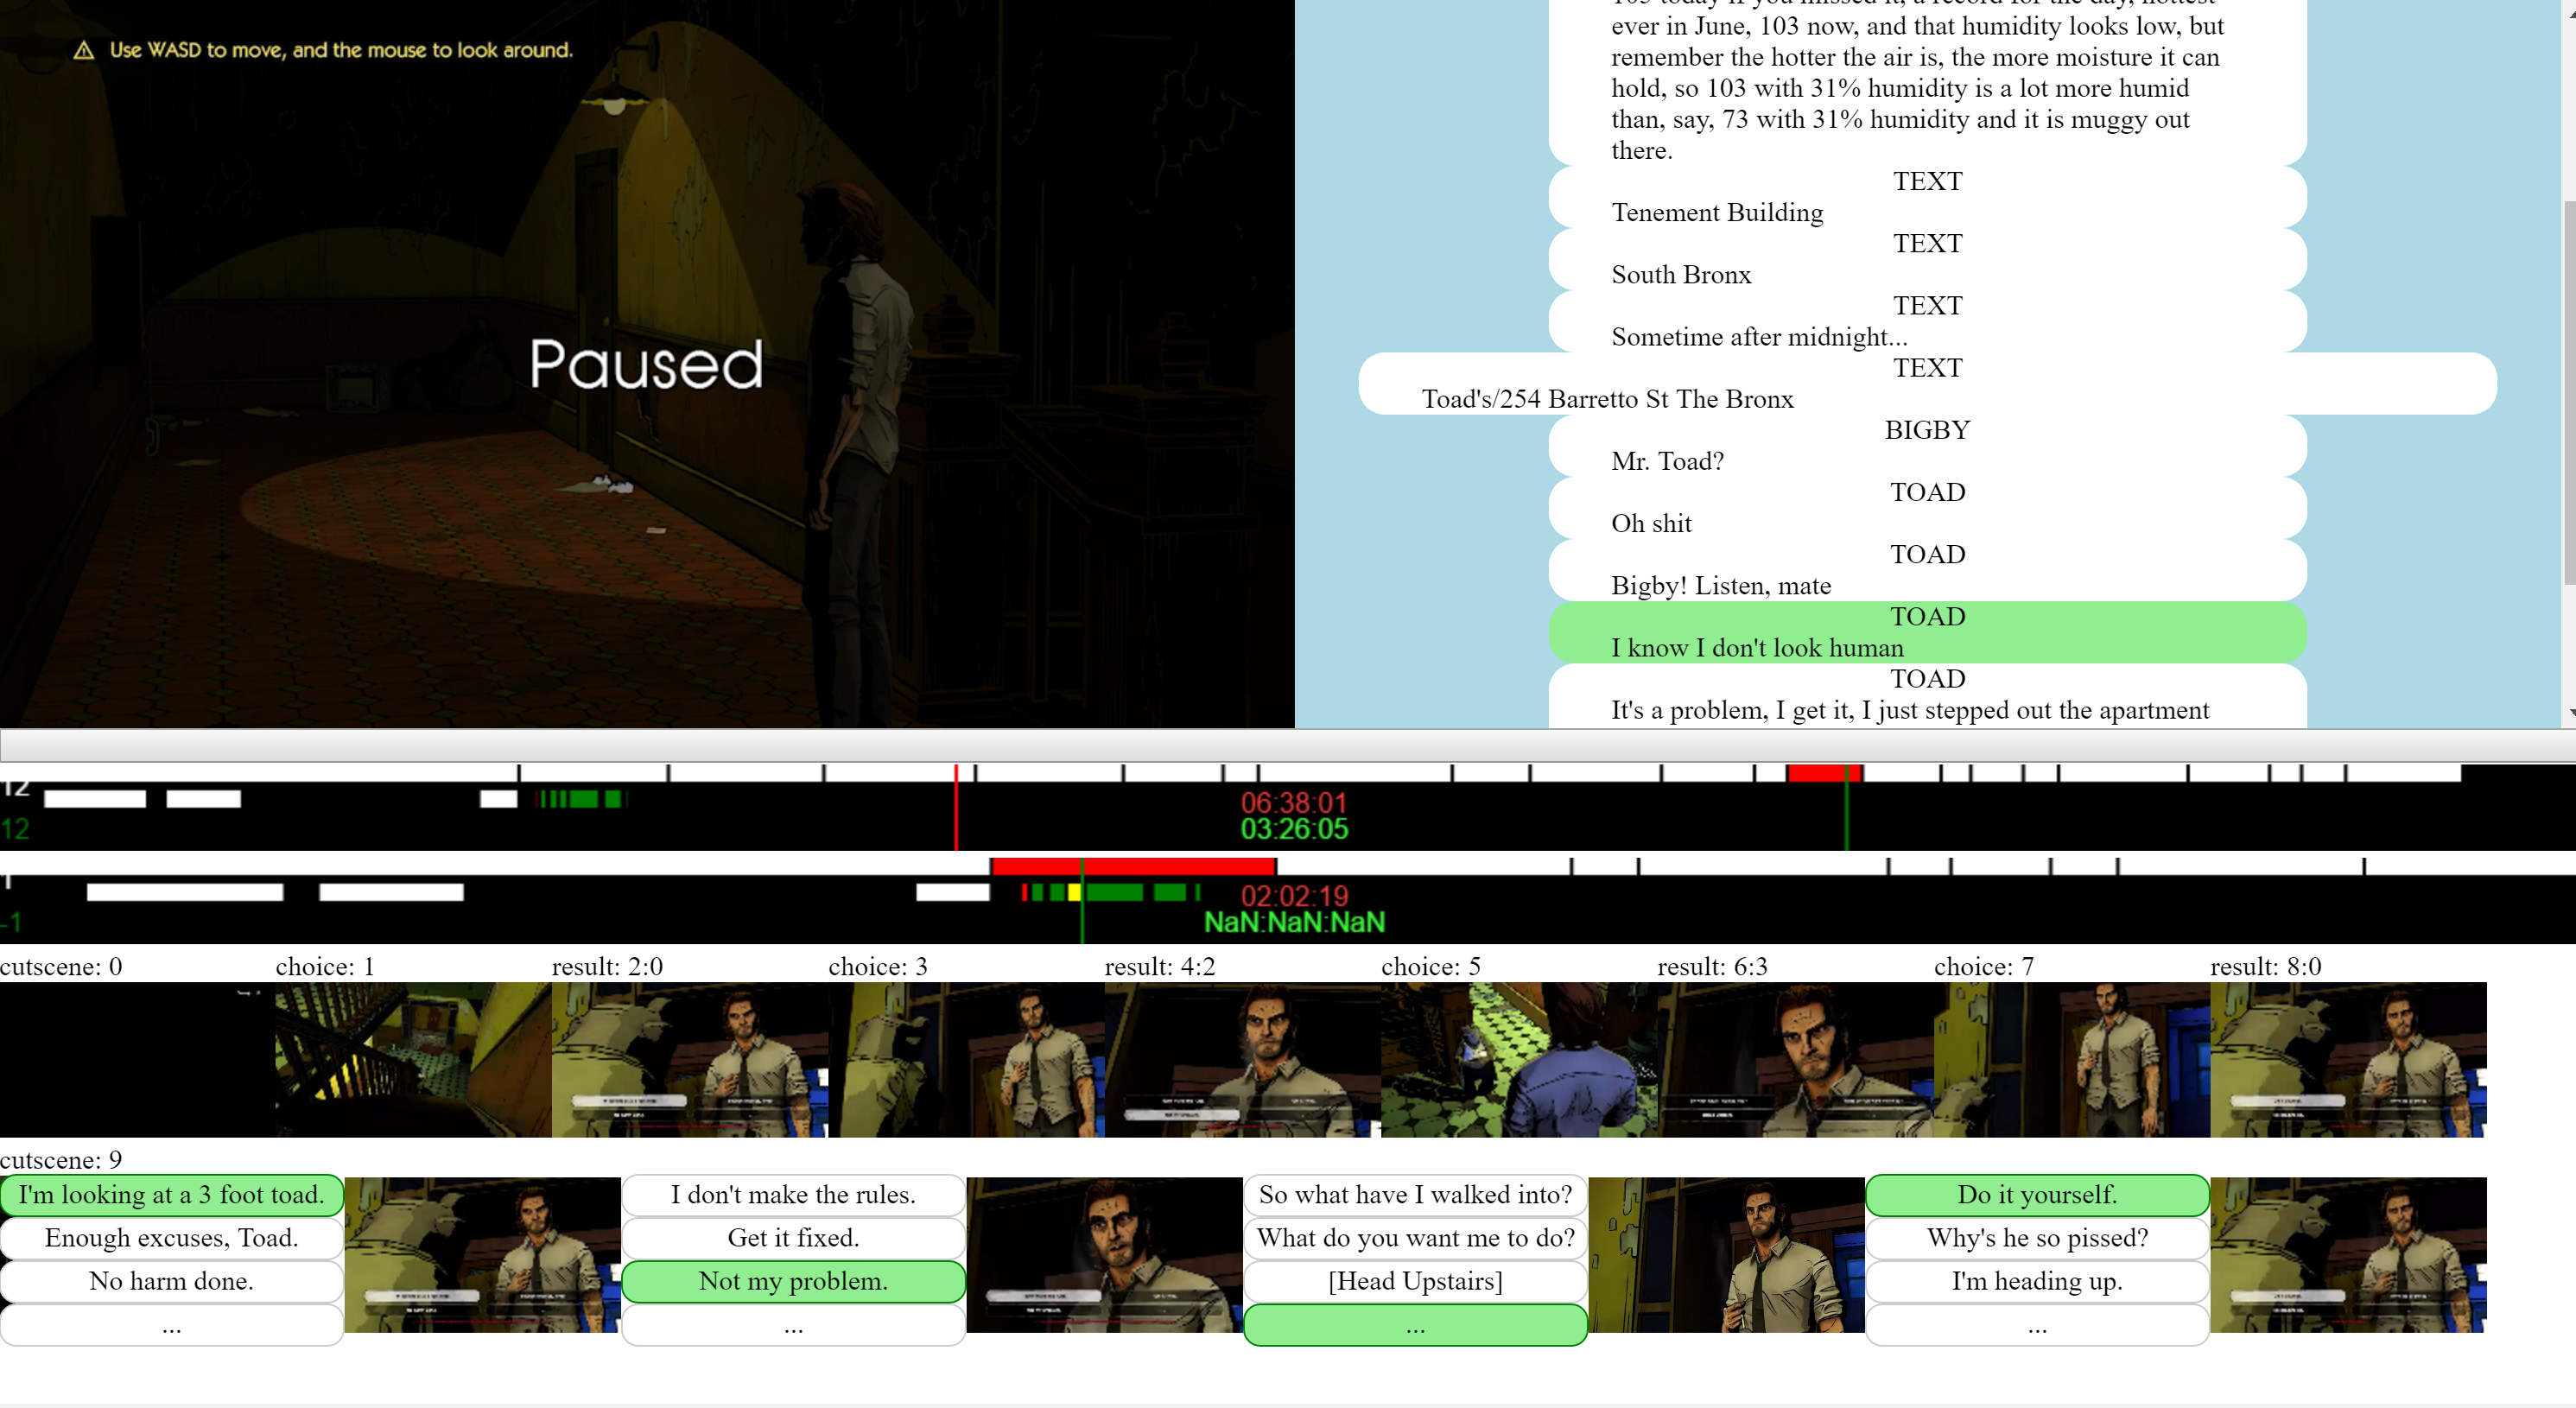
\includegraphics[width=10cm]{story_browser.png}
\caption{Story Browser Prototype Interface}
\end{figure}

The Story Browser Interface shows off two main features that would be
useful in analyzing and exploring surface traversals:

\begin{enumerate}
\item A navigation timeline that shows the location of segments of
content. In this version, there are two timelines. The first
represents the raw content (divided into segments corresponding
roughly to choice points and "cutscenes"
\item A choice selection interface which allows the user to specify which
traversal to make "selected." Each choice point's options are
displayed along with the segment that results, changing to the
correct clip when the user selects the corresponding choice.
\end{enumerate}

For the Story Browser prototype, the encoding of the surface content
was performed manually. Non-linear video editing tools such as Adobe
Premier Pro are an inspiration for dealing with non-textual
content. These tools enable precise editing using operations such as
inserting a cut (a segmentation of a video file based on a timecode
that specifies a location for potential insertion of another clip.

In the current form, the content is recorded as segments reflecting
their variation, but it is anticipated that increasing the granularity
by adding shot-level metadata would better provide for comparisons
between different traversals in terms of which shots and lines of
dialogue are identical.

\section{Proposed Evaluation}
\label{sec:orgheadline16}
This encoding and prototype is based on an analysis of only a portion
of the target work, and future work depends on a complete encoding of
the entirety of the work using the proposed encoding. But we will
revisit the initial research question to propose how an encoding would
be evaluated.

\begin{quote}
How do you define and represent, using story control logics, the
significant story-related surface content of cinematic choice-based
adventure games?
\end{quote}

The question suggests several strategies for evaluation. The selection
of content types, relationships and metrics determine the types of
operations and questions which it can answer easily. Applying a set of
questions to the content, once encoded, would provide evidence that
the approach's utility is in revealing non-obvious answers about the
distribution of traversals and content that existing methods cannot.

Below are some examples of questions that engage with just the surface
story content itself:

\begin{itemize}
\item How much (in terms of percentage) of the content in \emph{The Wolf Among
Us} is displayed to a player on average? This requires a mechanistic
tabulation of the surface story content without any interpretation
or reference to SIG content, but would be useful in answering
questions about authorial burden or "efficiency" of the work's usage
of hand-authored content in a more precise way than lines of
dialogue.
\item What are the distributions of traversal length? Does traversal length,
measured by either content elements or total time, follow a normal
curve?
\item How can each decision be ranked in terms of its impact on the
possible traversals it is a precondition for?
\end{itemize}

By using elements traditionally analyzed by film to segment the work
and using the three "story control" operational logics (OL1, OL2, OL3,
OL4 and OL5), a number of questions which engage the material surface
could be formulated.  The answers can be strengthened by using the
surface content dataset and the visualizations and examples it would
highlight. An example of such a traversal could be one discovered
where the player-character has the shortest total traversal time as
measured by summing up the duration of each segment length. What
choices did the player make that gave rise to such a traversal? Were
they surprising in any way? How much do similar traversals vary, and
were there any indicators as to their significance in those dialogue
options?

\section*{Closing and Future Work}
\label{sec:orgheadline17}
Cinematic choice-based adventure games are popular and successful
non-linear narratives that are often seen as an anomaly in their
reliance on hand-authored content, but what they represent is an
opportunity to understand story and interactivity in a genre that is
potentially tractable for computational narratology approaches. This
paper described a surface encoding that would be a foundation for
future models of content, both using computer vision approaches that
utilize the metadata as well as approaches that seek to model the
story content, as David Elson accomplishes through the Story Intention
Graph schemata \cite{Elson2012}. By better understanding what
currently works as interactive narrative experiences using
computational methods, we can better understand both how to develop
better content and how existing artifacts create the effects that they
do.

\bibliographystyle{splncs03}
\bibliography{AdvancementProposal}
\end{document}
